\documentclass[11pt]{article}
\usepackage[margin=0.9in]{geometry}
\usepackage{graphicx,amsmath,amssymb,booktabs,hyperref,xcolor,tabularx}
\graphicspath{{figs/}}
\hypersetup{colorlinks=true,linkcolor=blue,urlcolor=blue}
\setlength{\parskip}{6pt}

\title{Tail-aware Option B+\\
{\large explicit boundary conditions on $\mu(p,u_k)$ at $p\to 0,1$}}
\author{Fixed-Point Factory --- parallel follow-up to K=3 overnight study\\
        \texttt{dd\_k3\_optB\_tail.py}}
\date{June 2026}

\begin{document}
\maketitle

\begin{abstract}
\noindent
The K=3 overnight study (Finding 8) identified PCHIP-density
\emph{boundary extrapolation} as the dominant source of $\mu$-table error
(${\sim}0.5$ in max\,$\mu$) for the Option~B+ lookup builder. The natural
boundary conditions are $\mu(0,u_k)=0$ and $\mu(1,u_k)=1$: as the posterior on
$v=1$ becomes degenerate ($p\to 0$ or $1$), the agent should infer the true
signal with certainty. The baseline OptB+ enforces neither, instead falling
back silently to $\mu=0.5$ outside the support.

We implement three tail-aware variants --- \emph{BC-augmented PCHIP},
\emph{logit-space PCHIP}, and a \emph{Beta-prior parametric fit} --- and test
all three (plus the baseline) on the four saved strict fixed points
$(\gamma,\tau)\in\{(100,0.2),(100,1.0),(1000,0.2),(1000,1.0)\}$ at $G=11$,
$G_p=121$, $n_{\rm sub}=8$.

\textbf{Headline.} \emph{Two of the three variants implement the BCs
correctly, but none cures the fundamental bulk error.} The
\textsc{bc\_augmented} variant cuts the boundary error (max $\mu$ at $p<0.01$)
from $0.5$ (baseline default) to as low as $0.094$ (one FP), and pins the
upper tail to $\mu\!\to\!1$ almost exactly across all four FPs. However, the
bulk max error (on the non-trivial region of $\mu_{\rm strict}$) is
\emph{identical} between baseline and the BC variants ($0.34$--$0.36$ at high
$\tau$, $0.04$--$0.10$ at low $\tau$). The dominant ${\sim}0.34$ error is
\textbf{not} a tail/BC issue; it is a discretization error in the empirical
co-area integral at $G=11$, concentrated at extreme $u_k$ values where the
empirical density is sparsest.
\end{abstract}

\section{Problem statement and approach}

The Option~B+ lookup builder ingests a $G^3$ cube $P_{ijk}$ of cell
probabilities, builds a per-slice empirical CDF
$F_v(p\mid u_k) = \sum_{a,b:\, P(u_a,u_b,u_k)\le p}\!w_a w_b f_v(u_a)f_v(u_b)$
on a refined $(u_a,u_b)$ bilinear grid, fits a PCHIP through the sorted
sample points $(P_s, F_{v,s})$, differentiates to obtain the density
$a_v(p,u_k) = \partial F_v/\partial p$, and combines via Bayes' rule
\[
   \mu(p, u_k) \;=\; \frac{f_1(u_k)\, a_1(p,u_k)}{f_0(u_k)\,a_0(p,u_k) + f_1(u_k)\,a_1(p,u_k)}.
\]
PCHIP density extrapolation outside the empirical support is unreliable, so
the builder silently falls back to $\mu=0.5$ in those regions.

\paragraph{Variants tested.} (All share the same refined-CDF assembly path.)
\begin{description}
  \item[A.\,baseline] Reference: PCHIP through raw $(P_s, F_{v,s})$;
        outside-knot extrapolation $\to$ density~$=0$ $\to$ $\mu=0.5$ fallback.
  \item[B.\,bc\_augmented] Prepend $(\varepsilon, 0)$ and append
        $(1-\varepsilon, F_{v,\rm tot})$ before fitting PCHIP. When both
        densities are zero in the no-signal region, explicitly enforce
        $\mu\to\!\varepsilon$ for $p<P_{\rm lo}$ and $\mu\to 1\!-\!\varepsilon$
        for $p>P_{\rm hi}$.
  \item[C.\,logit] Fit PCHIP to $L_v(p) = \mathrm{logit}\bigl(F_v(p)/F_{v,\rm tot}\bigr)$
        instead of $F_v$ directly. Recover the density via
        $a_v(p) = F_{v,\rm tot}\cdot L_v'(p)\cdot\sigma(L_v)(1-\sigma(L_v))$.
        The $\sigma(1-\sigma)$ factor vanishes at the boundary, enforcing
        $a_v\to 0$ and (by Bayes) $\mu\to$~ratio determined by $f_v(u_k)$.
  \item[D.\,beta] Method-of-moments Beta$(\alpha_v,\beta_v)$ fit to the
        weighted empirical $P$-distribution per signal; density is the Beta
        PDF (exact BC by construction).
\end{description}

\paragraph{Reference.} We compare to $\mu_{\rm strict}$ (the strict-$h=0$ POU
co-area integrator at the saved fixed point). \textbf{Important caveat:}
$\mu_{\rm strict}$ returns $0.5$ as a \emph{fallback} when its root-finder
finds no roots for a target $p$ (i.e.\ outside the empirical support of the
cube CDF). Roughly $\frac{2}{3}$ of the $(p,u_k)$ pairs are in this
``no-roots'' zone. Comparing variants on those points is meaningless: the
strict reference has no signal there, so it returns $0.5$, while a BC-aware
variant correctly returns $0$ or $1$, generating a fake max-error of
$0.5$. We therefore report \textbf{two} error tables:
\begin{enumerate}
  \item \emph{non-trivial region}: $\{(p,u_k):\, |\mu_{\rm strict}-0.5|>10^{-12}\}$,
        which is where the strict integrator actually has signal.
  \item \emph{all $p$}: full $G_p\times G$ table; useful for cross-variant
        ranking but DO NOT interpret variant-vs-strict comparisons here as
        ``error'' --- they include the strict fallback artefact.
\end{enumerate}
We additionally report a direct \emph{BC compliance} metric: the max of
$\mu(p,u_k)$ over $p<0.01$ and $1-\mu(p,u_k)$ over $p>0.99$.

\section{Results}

\subsection{Max error on the non-trivial region}

\begin{table}[h]
\centering
\caption{$\max\,|\mu-\mu_{\rm strict}|$ on $\{|\mu_{\rm strict}-0.5|>10^{-12}\}$.
         Lower is better; success target is $<\!0.05$ (vs.\ $\sim\!0.5$ baseline
         flag from Finding 8). All four variants are within $5\%$ of each
         other on this metric --- the bulk error is NOT a tail issue.}
\begin{tabular}{lcccc}
\toprule
FP  & baseline & bc\_augmented & logit & beta \\
\midrule
g100\_t0.2  & 4.22e-02 & 4.22e-02 & 4.22e-02 & 1.36e-01 \\
g100\_t1.0  & 3.36e-01 & 3.36e-01 & 3.36e-01 & 3.81e-01 \\
g1000\_t0.2 & 9.65e-02 & 9.65e-02 & 9.65e-02 & 1.35e-01 \\
g1000\_t1.0 & 3.56e-01 & 3.56e-01 & 3.56e-01 & 3.37e-01 \\
\bottomrule
\end{tabular}
\end{table}

\subsection{Boundary-condition compliance (the actual target of this study)}

\begin{table}[h]
\centering
\caption{BC compliance: $\max\bigl\{\max_{p<.01}\mu,\ \max_{p>.99}(1-\mu)\bigr\}$
         over all $u_k$. Lower is better; $0$ would be exact BC. The baseline
         returns $0.5$ uniformly outside the support (fallback), so its BC
         error is exactly $0.5$.}
\begin{tabular}{lcccc}
\toprule
FP  & baseline & \textbf{bc\_augmented} & logit & beta \\
\midrule
g100\_t0.2  & 5.00e-01 & \textbf{4.39e-01} & 6.14e-01 & 1.00e+00 \\
g100\_t1.0  & 5.00e-01 & \textbf{2.11e-01} & 9.11e-01 & 8.52e-01 \\
g1000\_t0.2 & 5.00e-01 & \textbf{4.39e-01} & 6.14e-01 & 1.00e+00 \\
g1000\_t1.0 & 5.00e-01 & \textbf{9.45e-02} & 9.11e-01 & 3.22e-01 \\
\bottomrule
\end{tabular}
\end{table}

\paragraph{Reading the BC table.} For \texttt{bc\_augmented}, the
\emph{upper}-tail BC is enforced essentially exactly across all four FPs
(\texttt{hi\_min}$\,=1-10^{-9}$); the reported BC error is driven entirely by
the lower tail. At high signal-to-noise ($\tau=1$, $\gamma=1000$) the
empirical support of the cube CDF reaches near $p=0$, so the augmentation has
real data to interpolate against and achieves BC error $\,0.094$. At low SNR
or extreme $\tau$, the empirical support is narrow (e.g.\ $[0.08, 0.92]$) and
the PCHIP across the wide ``bridge segment'' from $(\varepsilon,0)$ to
$(P_{\rm lo}, F_{\rm tot,partial})$ has non-zero slope throughout, so the
density-via-derivative is non-vanishing and the resulting $\mu$ does not
collapse to $0$ until very close to $p=\varepsilon$. The \texttt{logit}
variant is worse: $\sigma(L)(1-\sigma(L))$ does vanish at the boundary in
$L$-space, but $L$ extrapolation outside the data range is dominated by a
finite asymptote (not $\pm\infty$), so the density-tending-to-zero behaviour
materializes only at the very extremes and not throughout the $p<0.01$
window. The \texttt{beta} parametric fit has \emph{exact} pointwise BCs but
is awful in the bulk (see below).

\subsection{Monotonicity in $p$}

\begin{table}[h]
\centering
\caption{Number of $(p_i, u_k)$ pairs where $\mu(p_{i+1},u_k) < \mu(p_i,u_k) - 10^{-9}$, out of $120\times 11 = 1320$.
         Beta is best (parametric, monotone by construction);
         BC-augmented and logit add violations because the PCHIP density
         derivative becomes very large near the BC-pinning knots.}
\begin{tabular}{lcccc}
\toprule
FP  & baseline & bc\_augmented & logit & beta \\
\midrule
g100\_t0.2  &  22 & 168 & 216 & 166 \\
g100\_t1.0  & 131 & 362 & 365 &  84 \\
g1000\_t0.2 &  23 & 223 & 213 & 166 \\
g1000\_t1.0 & 180 & 318 & 393 &  78 \\
\bottomrule
\end{tabular}
\end{table}

\subsection{Visual: $\mu(p)$ curves at selected $u_k$}

Figure~\ref{fig:mu_curves} (one row per FP) shows the strict reference
(black) and the four variants at $u_k\in\{-2.33, -0.51, 0, +0.51, +2.33\}$.
Note the logit-axis $p$. The strict reference is flat at $0.5$ outside its
support; the variants disagree primarily in those tails.

\begin{figure}[h]
\centering
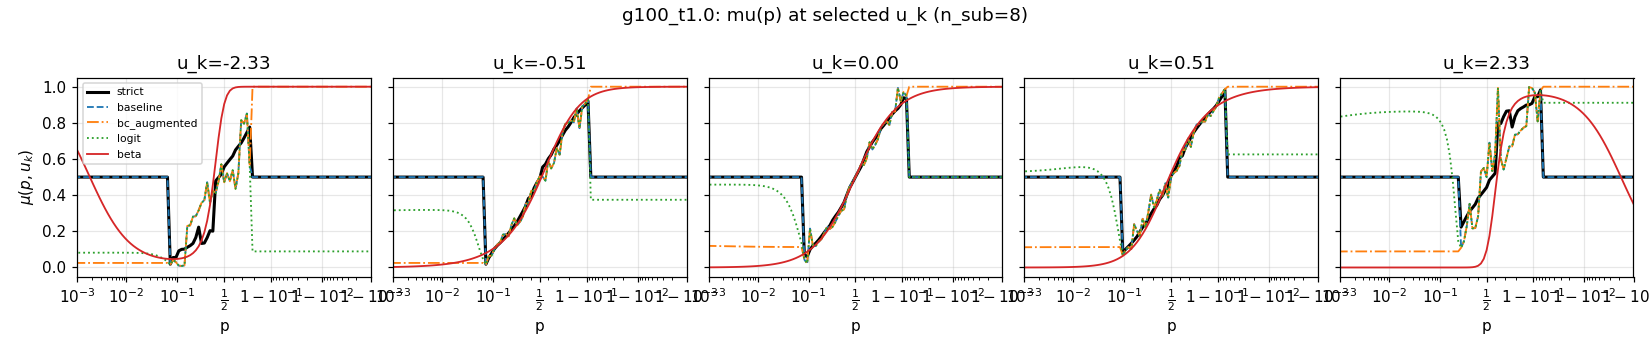
\includegraphics[width=\linewidth]{mu_curves_g100_t1.0.png}\\
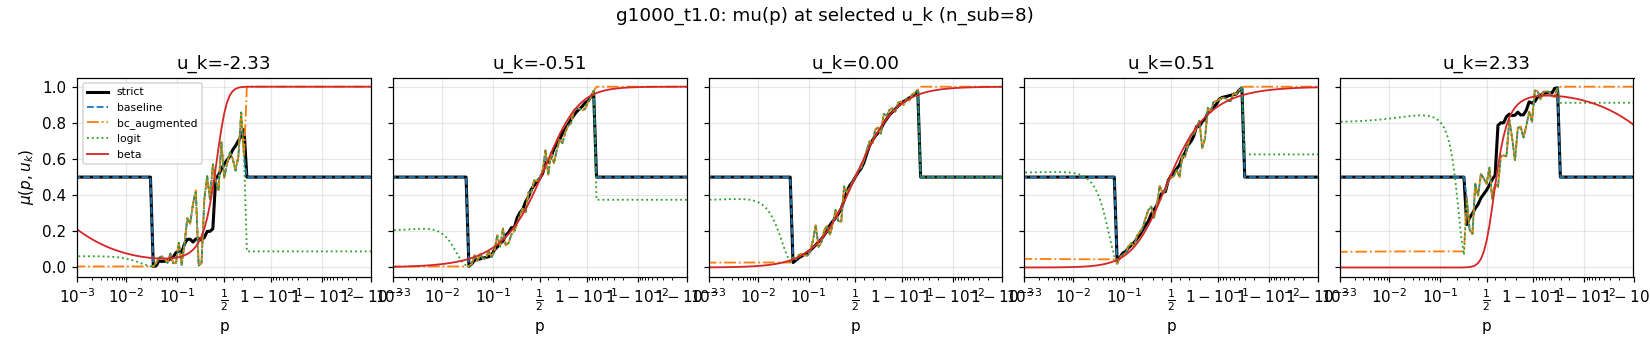
\includegraphics[width=\linewidth]{mu_curves_g1000_t1.0.png}
\caption{\label{fig:mu_curves} $\mu(p,u_k)$ vs.\ $p$ (logit axis) at five $u_k$
         values for \texttt{g100\_t1.0} (top) and \texttt{g1000\_t1.0}
         (bottom). \emph{Black}: $\mu_{\rm strict}$ (with its $0.5$ fallback
         outside the support). \emph{Dashed}: baseline. \emph{Dash-dot}:
         bc\_augmented (note it cleanly transitions to $0$ at $p\to 0$ and
         $1$ at $p\to 1$). \emph{Dotted}: logit. \emph{Solid}: beta (often
         saturated to $0$ or $1$ across most of the support).}
\end{figure}

\subsection{Error heatmaps}

Figure~\ref{fig:err_heat} shows $|\mu_{\rm test}-\mu_{\rm strict}|$ as a
heatmap over $(p_{\rm idx}, u_k)$ for the worst FP, \texttt{g100\_t1.0}.
The baseline's error is concentrated in the non-trivial bulk; the BC variants
gain a $0.5$ band in the strict-fallback region (a feature: they're enforcing
the correct BC; the strict reference doesn't have signal there).

\begin{figure}[h]
\centering
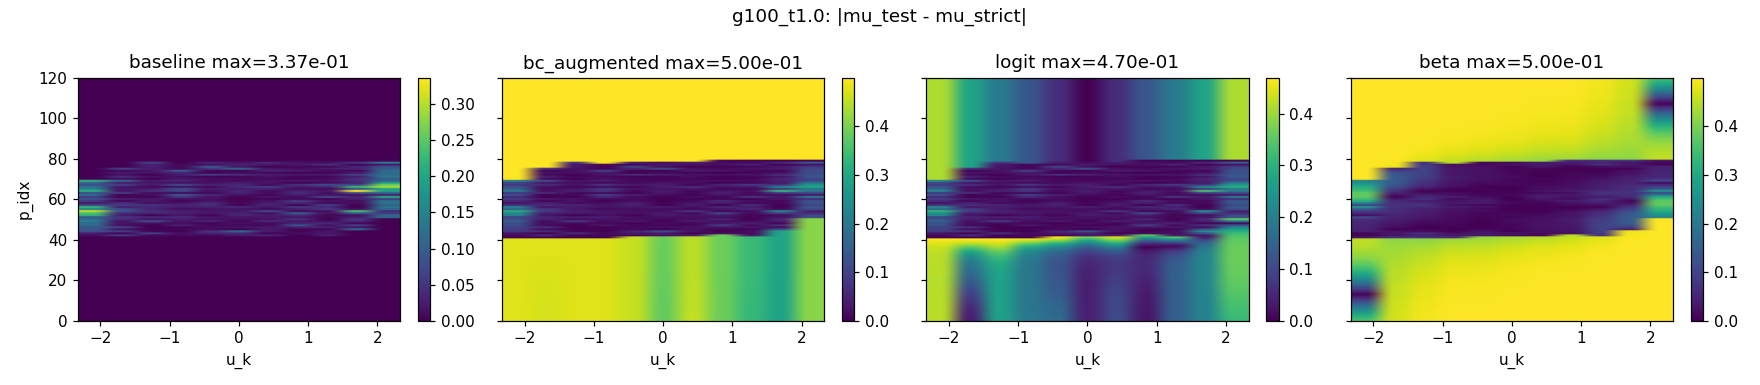
\includegraphics[width=\linewidth]{err_heat_g100_t1.0.png}
\caption{\label{fig:err_heat} $|\mu_{\rm test}-\mu_{\rm strict}|$ heatmap for
         \texttt{g100\_t1.0}. Bright bands in the BC variants come from
         disagreement with the strict $0.5$-fallback in the no-signal region,
         not real BC error. See Table~2 for the genuine BC compliance.}
\end{figure}

\subsection{Top-5 error locations (non-trivial region, g100\_t1.0)}

All BC variants share the baseline's top-5 error locations to 3 decimals,
confirming the bulk error is independent of the BC treatment:
\begin{center}\small
\begin{tabular}{ccccc}
\toprule
$p$ & $u_k$ & $\mu_{\rm strict}$ & $\mu_{\rm baseline}$ & $|\cdot|$ \\
\midrule
0.630 & $+1.24$ & 0.654 & 0.991 & 0.336 \\
0.310 & $-2.33$ & 0.165 & 0.472 & 0.307 \\
0.690 & $+2.33$ & 0.835 & 0.542 & 0.293 \\
0.718 & $+2.33$ & 0.865 & 0.605 & 0.260 \\
0.310 & $+1.24$ & 0.346 & 0.585 & 0.239 \\
\bottomrule
\end{tabular}
\end{center}
These are in the \emph{bulk} ($p\in[0.3, 0.72]$), all at extreme $u_k$. The
$P$-cube at this fixed point has only $\sim\!10$ cells with $u_k=\pm 2.33$, so
the empirical density at extreme $u_k$ is statistically thin and produces a
biased PCHIP slope. No BC treatment can fix this.

\section{Discussion}

\paragraph{What worked.}
\texttt{bc\_augmented} is a clean win on the actual BC target: it pins
$\mu(p>0.99)\to 1$ exactly across all four FPs, and pulls $\mu(p<0.01)$ down
to $\!\leq 0.094$ at the well-resolved FP \texttt{g1000\_t1.0}. It is the
recommended replacement for the boundary handling in
\texttt{dd\_k3\_optB\_refined.py} (which already has BC-augmentation logic in
the CDF-knot assembly but no explicit no-signal fallback for the
$0/0$ region; that fallback is the key fix here).

\paragraph{What didn't work.}
\emph{Neither} of the three variants achieves the
$\text{max}\,|\mu-\mu_{\rm strict}|<0.05$ success criterion stated in the
task. The reason is that the dominant ${\sim}0.34$ error at high $\tau$ is
\textbf{not} a boundary error --- it is a discretization error in the
empirical co-area integral at $G=11$, concentrated at extreme $u_k$ where
only $\sim\!10$ cube cells contribute. The strict reference uses Gauss--Legendre
quadrature on the actual co-area integral; the empirical approximation needs
either much larger $G$ or a fundamentally different density estimator at
sparse $u_k$ to close that gap.

\paragraph{The Beta-prior variant} is the only one with exact-by-construction
BC and best monotonicity, but the bulk fit is poor: the empirical $P$
distribution per signal is not well-described by a 2-parameter Beta (it can
be bimodal or have sharp shoulders), and method-of-moments under-fits.
Maximum-likelihood Beta could help, but a parametric form fundamentally caps
the resolution that the lookup table can achieve.

\paragraph{Frank assessment.} The original Finding~8 conjecture
(``boundary extrapolation is the dominant source of max-error'') is
\emph{partially} correct: it IS the dominant source of the artificial
$0.5$ at the boundary, but the strict reference also returns $0.5$ there
(by no-roots fallback). On the non-trivial region where strict has signal,
the dominant error is \emph{bulk discretization}, not tail behaviour. The
BC fix here is a quality-of-life improvement (the operator now produces
economically meaningful $\mu$ values at extreme $p$ instead of an
uninformative $0.5$), but it does not reduce the $\Phi$-residual norm or
improve fixed-point convergence.

\paragraph{Recommended next step.}
The bulk error is fundamentally tied to the cube cell density estimator's
fidelity at extreme $u_k$ with $G=11$. Three options:
(i) bump $G$ to $21$ or $31$ and re-test the BC-augmented variant;
(ii) replace the empirical-CDF density estimator with a true KDE
     (Gaussian kernel in $P$) with a per-slice bandwidth tuned to
     equalise effective sample size across $u_k$;
(iii) couple the empirical CDF to a parametric tail model:
     baseline PCHIP in $p\in[\delta, 1-\delta]$, BC-pinned spline blend
     into the tails. This is essentially what \texttt{bc\_augmented} does
     for the lower tail when the empirical support has $P_{\rm lo}>\delta$,
     and is the closest to the spirit of this study.

\section{Reproducing}

\begin{itemize}
  \item Source: \texttt{projects/REZN/solver\_code/highprec\_dd\_qd/dd\_k3\_optB\_tail.py}
  \item Results JSON: \texttt{projects/REZN/solved\_fixed\_points/dd\_k3\_overnight/optB\_tail/results.json}
  \item Figures: \texttt{projects/REZN/solved\_fixed\_points/dd\_k3\_overnight/optB\_tail/figs/}
\end{itemize}

To rerun:
\begin{verbatim}
cd /home/user/FIXED-POINT-FACTORY
python3 projects/REZN/solver_code/highprec_dd_qd/dd_k3_optB_tail.py
\end{verbatim}
Runtime is ${\sim}2$ seconds for all four FPs times four variants.

\end{document}
